\section{BeispielCode}
\subsection{FlipFlop}
\lstinputlisting[ title=Flip Flop]{code/example/FlipFlop.vhd}

\subsection{Synchrone Freigabe}
\lstinputlisting[ title=Synchrone Freigabe]{code/example/Sync_en.vhd}

\subsection{Metastabilitätsfilter Synchronistation}
\lstinputlisting[ title=Synchronistation]{code/example/synch.vhd}

\subsection{Entprellen}
Schalter und Taster können auf zwei Arten entprellt werden.\\
\begin{itemize}
\item Unterabtasten
\item Wartezeit Blanktime
\end{itemize}
\lstinputlisting[ title=Entprellen]{code/example/Entprellen.vhd}

\subsection{4 zu 1 Mulitplexer}

\subsubsection{Multiplexer Code Using if else statements}
Der 4 to 1 Multiplexer wird auf vier verschiedene Prozessarten gelöst.
\lstinputlisting[ title=Mux]{code/example/4to1Mux.vhd}

\subsection{FSM}

\subsubsection{Schloss mit Schieberegister ohne FSM}
\lstinputlisting[ title=Schloss ohne FSM]{code/example/schloss_shift.vhd}

\subsubsection{Schloss mit FSM}
\lstinputlisting[ title=Schloss mit FSM]{code/example/schloss_fsm.vhd}

\subsubsection{Schloss mit FSM, Metastabilitätsfilter und Entprellung}
\lstinputlisting[ title=Schloss mit FSM\, Metastabilitätsfilter und Entprellung]{code/example/schloss_fsm_debounce.vhd}

%------------------------------------------------------------------------
%Mealy FSM mit Bild
\newpage
\subsubsection{Mealy FSM}
\lstinputlisting[ title=Mealy FSM]{code/example/fsm_mealy.vhd}

\begin{figure}[htbp]
	\centering
		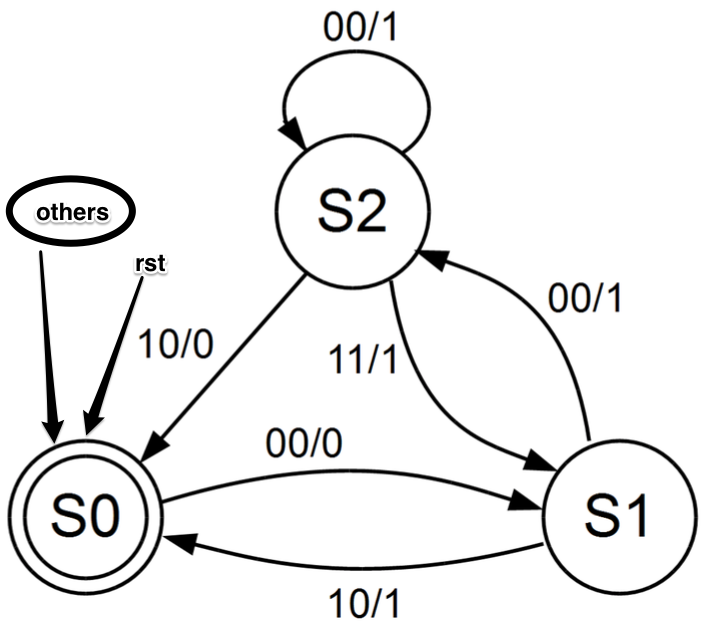
\includegraphics[width=5cm]{content/bilder/fsm_mealy.png}
	\caption{Sequenzdiagramm des Mealy Automaten}%
	\label{Mealy}
\end{figure}

%------------------------------------------------------------------------
%Moore FSM mit Bild
\newpage
\subsubsection{Moore FSM}
\lstinputlisting[ title=Moore FSM]{code/example/fsm_moore.vhd}

\begin{figure}[htbp]
	\centering
		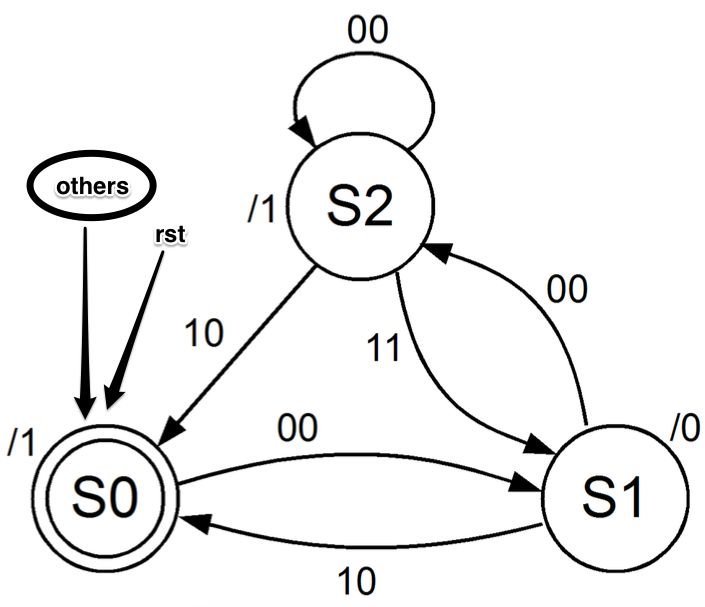
\includegraphics[width=5cm]{content/bilder/fsm_moore.png}
	\caption{Sequenzdiagramm des Moore Automaten}%
	\label{Moore}
\end{figure}
